\begin{figure}
    \centering
    

\tikzset{every picture/.style={line width=0.75pt}} %set default line width to 0.75pt        

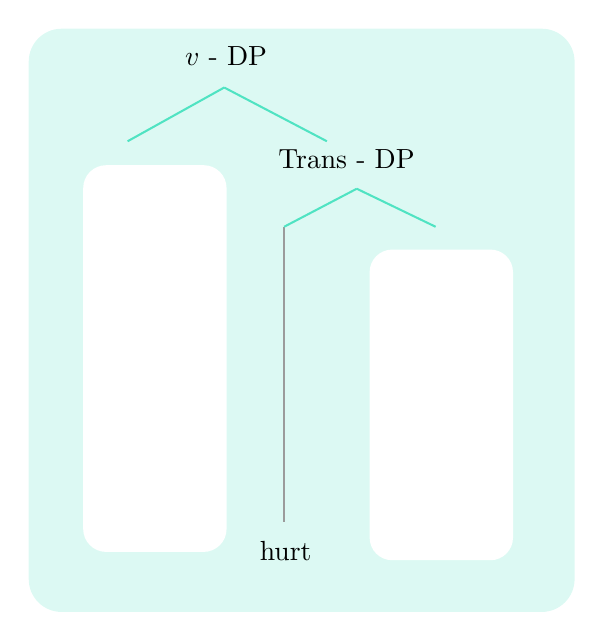
\begin{tikzpicture}[x=0.75pt,y=0.75pt,yscale=-1,xscale=1]
%uncomment if require: \path (0,300); %set diagram left start at 0, and has height of 300

%Rounded Rect [id:dp6179629271510167] 
\draw  [draw opacity=0][fill={rgb, 255:red, 80; green, 227; blue, 194 }  ,fill opacity=0.2 ] (264,21.22) .. controls (264,12.48) and (271.08,5.4) .. (279.82,5.4) -- (511.18,5.4) .. controls (519.92,5.4) and (527,12.48) .. (527,21.22) -- (527,270.58) .. controls (527,279.32) and (519.92,286.4) .. (511.18,286.4) -- (279.82,286.4) .. controls (271.08,286.4) and (264,279.32) .. (264,270.58) -- cycle ;
%Straight Lines [id:da5124281058149747] 
\draw [color={rgb, 255:red, 155; green, 155; blue, 155 }  ,draw opacity=1 ]   (387.05,100.83) -- (387.05,243) ;
%Straight Lines [id:da45639078775028685] 
\draw [color={rgb, 255:red, 80; green, 227; blue, 194 }  ,draw opacity=1 ]   (460.05,100.83) -- (422.05,82.5) ;
%Straight Lines [id:da8054931432940027] 
\draw [color={rgb, 255:red, 80; green, 227; blue, 194 }  ,draw opacity=1 ]   (422.05,82.5) -- (387.05,100.83) ;
%Straight Lines [id:da5421084389764239] 
\draw [color={rgb, 255:red, 80; green, 227; blue, 194 }  ,draw opacity=1 ]   (407.65,59.63) -- (358.2,33.73) ;
%Straight Lines [id:da49237182503455457] 
\draw [color={rgb, 255:red, 80; green, 227; blue, 194 }  ,draw opacity=1 ]   (358.2,33.73) -- (311.65,59.63) ;
%Rounded Rect [id:dp20189799754335946] 
\draw  [draw opacity=0][fill={rgb, 255:red, 255; green, 255; blue, 255 }  ,fill opacity=1 ] (428.24,122.7) .. controls (428.24,116.69) and (433.12,111.81) .. (439.14,111.81) -- (486.44,111.81) .. controls (492.46,111.81) and (497.33,116.69) .. (497.33,122.7) -- (497.33,250.59) .. controls (497.33,256.6) and (492.46,261.48) .. (486.44,261.48) -- (439.14,261.48) .. controls (433.12,261.48) and (428.24,256.6) .. (428.24,250.59) -- cycle ;
%Rounded Rect [id:dp5406671263937812] 
\draw  [draw opacity=0][fill={rgb, 255:red, 255; green, 255; blue, 255 }  ,fill opacity=1 ] (290.24,82.23) .. controls (290.24,76.11) and (295.21,71.15) .. (301.33,71.15) -- (348.24,71.15) .. controls (354.37,71.15) and (359.33,76.11) .. (359.33,82.23) -- (359.33,246.39) .. controls (359.33,252.51) and (354.37,257.48) .. (348.24,257.48) -- (301.33,257.48) .. controls (295.21,257.48) and (290.24,252.51) .. (290.24,246.39) -- cycle ;

% Text Node
\draw (387.76,263) node [anchor=south] [inner sep=0.75pt]   [align=left] {hurt};
% Text Node
\draw (382.8,61.92) node [anchor=north west][inner sep=0.75pt]   [align=left] {Trans - DP};
% Text Node
\draw (337.8,12.72) node [anchor=north west][inner sep=0.75pt]   [align=left] {$\displaystyle v$ - DP};


\end{tikzpicture}

\caption{A pre-compiled $v$P tree with two slots}
\end{figure}